Если заменить положительный окуляр астрономической трубы отрицательным, получается галилеева 
(или земная) труба. При телескопическом ходе лучей в галилеевой трубе расстояние между объективом 
и окуляром равно разности 

\begin{figure}[h]
  \center{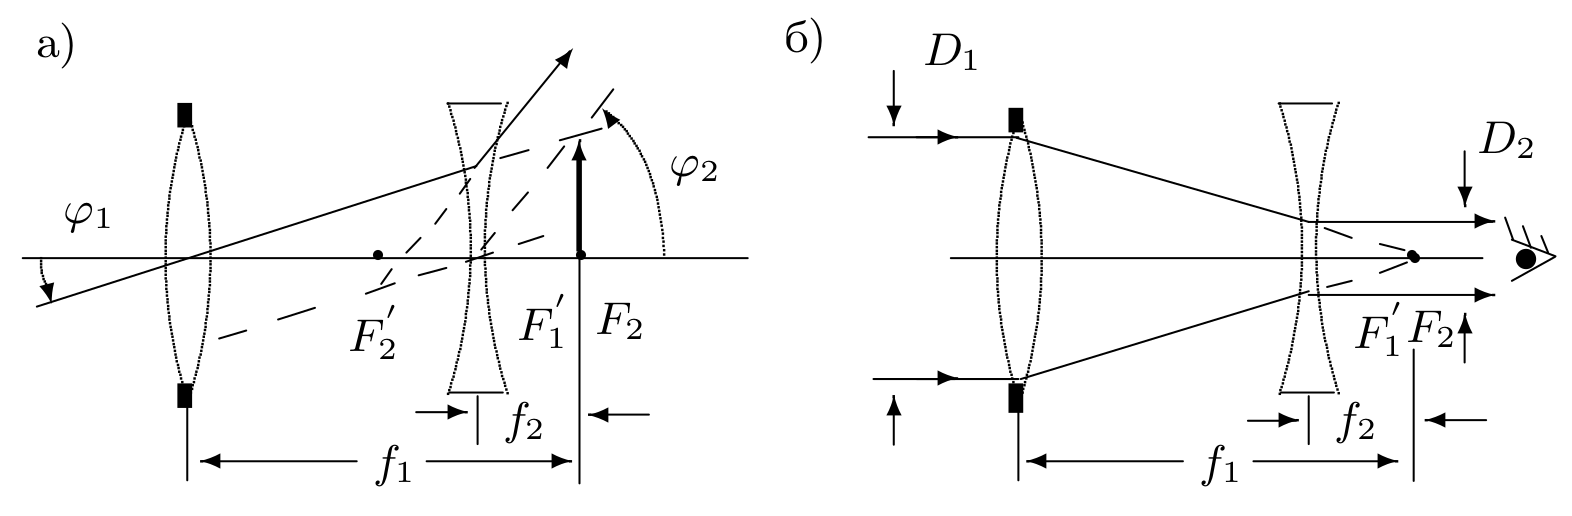
\includegraphics[width=\linewidth]{5.png}}
  \caption{К расчёту увеличения галилеевой зрительной трубы}
  \label{img::5}
\end{figure}

\noindent (точнее - алгебраической сумме) их фокусных расстояний (рис. \ref{img::5}), а
изображение оправы объектива, даваемое окуляром, оказывается мнимым. Это изображение располагается 
между объективом и окуляром. Легко показать, что формула \eqref{eq::4}), полученная для 
астрономической трубы, справедлива и для земной трубы.

Достоинством галилеевой трубы является то, что она даёт прямое
изображение. Поэтому зрительные трубы, бинокли и т.д. делаются по
схеме Галилея.